\documentclass[
	% -- opções da classe memoir --
	12pt,				% tamanho da fonte
	openright,			% capítulos começam em pág ímpar (insere página vazia caso preciso)
	oneside,			% para impressão em verso e anverso. Oposto a oneside
	a4paper,			% tamanho do papel. 
	% -- opções da classe abntex2 --
	%chapter=TITLE,		% títulos de capítulos convertidos em letras maiúsculas
	%section=TITLE,		% títulos de seções convertidos em letras maiúsculas
	%subsection=TITLE,	% títulos de subseções convertidos em letras maiúsculas
	%subsubsection=TITLE,% títulos de subsubseções convertidos em letras maiúsculas
	% -- opções do pacote babel --
	english,			% idioma adicional para hifenização
	french,				% idioma adicional para hifenização
	spanish,			% idioma adicional para hifenização
	brazil				% o último idioma é o principal do documento
	]{abntex2}

% ---
% Pacotes básicos 
% ---
\usepackage{lmodern}			% Usa a fonte Latin Modern			
\usepackage[T1]{fontenc}		    % Selecao de codigos de fonte.
\usepackage[utf8]{inputenc}		% Codificacao do documento (conversão automática dos acentos)
\usepackage{lastpage}			% Usado pela Ficha catalográfica
\usepackage{indentfirst}		    % Indenta o primeiro parágrafo de cada seção.
\usepackage{color}				% Controle das cores
\usepackage{graphicx}			% Inclusão de gráficos
\usepackage{microtype} 			% Para melhorias de justificação
\usepackage{afterpage}
\usepackage{amsmath}            % Pacote para fórmulas matemáticas
\usepackage{amssymb,url}
\usepackage{xcolor,tikz,bm,colortbl}
\usepackage[br]{nicealgo}       % Pacote para criação de algoritmos
\usepackage{customizacoes}

% ---
		
% ---
% Pacotes adicionais, usados apenas no âmbito do Modelo Canônico do abnteX2
% ---
\usepackage{lipsum}				% Para geração de dummy text
% ---

% ---
% Pacotes de citações
% ---
\usepackage[brazilian,hyperpageref]{backref}	 % Paginas com as citações na bibl
\usepackage[alf]{abntex2cite}	% Citações padrão ABNT
% --- 
% CONFIGURAÇÕES DE PACOTES
% --- 

% ---
% Configurações do pacote backref
\renewcommand{\familydefault}{\sfdefault}
% Usado sem a opção hyperpageref de backref
\renewcommand{\backrefpagesname}{Citado na(s) página(s):~}
% Texto padrão antes do número das páginas
\renewcommand{\backref}{}
% Define os textos da citação
\renewcommand*{\backrefalt}[4]{
	\ifcase #1 %
		Nenhuma citação no texto.%
	\or
		Citado na página #2.%
	\else
		Citado #1 vezes nas páginas #2.%
	\fi}%
% ---

% ---
% Informações de dados para CAPA e FOLHA DE ROSTO
% ---
\titulo{Aplicativo web para análise e comparação de Audio Fingerprint}
\autor{Evandro Barbosa Carreira}
\local{Bauru}
\data{2015}
\orientador{Prof. Dr. João Fernando Marar}
\instituicao{%
  Universidade Estadual Paulista ``Júlio de Mesquita Filho''
  \par
  Faculdade de Ciências
  \par
  Ciência da Computação}
\tipotrabalho{Trabalho de Conclusão de Curso}
% O preambulo deve conter o tipo do trabalho, o objetivo, 
% o nome da instituição e a área de concentração 
\preambulo{Trabalho de Conclusão de Curso do Curso de Ciência da Computação da Universidade Estadual Paulista ``Júlio de Mesquita Filho'', Faculdade de Ciências, Campus Bauru.}
% ---


% ---
% Configurações de aparência do PDF final

% alterando o aspecto da cor azul
\definecolor{blue}{RGB}{41,5,195}

% informações do PDF
\makeatletter
\hypersetup{
     	%pagebackref=true,
		pdftitle={\@title}, 
		pdfauthor={\@author},
    	pdfsubject={\imprimirpreambulo},
	    pdfcreator={LaTeX with abnTeX2},
		pdfkeywords={abnt}{latex}{abntex}{abntex2}{trabalho acadêmico}, 
		colorlinks=true,       		% false: boxed links; true: colored links
    	linkcolor=black,          	% color of internal links
    	citecolor=black,        		% color of links to bibliography
    	filecolor=magenta,      		% color of file links
		urlcolor=black,
		bookmarksdepth=4
}
\makeatother
% --- 

% --- 
% Espaçamentos entre linhas e parágrafos 
% --- 

% O tamanho do parágrafo é dado por:
\setlength{\parindent}{1.3cm}

% Controle do espaçamento entre um parágrafo e outro:
\setlength{\parskip}{0.2cm}  % tente também \onelineskip

% ---
% compila o indice
% ---
\makeindex
% ---

% ----
% Início do documento
% ----
\begin{document}

% Seleciona o idioma do documento (conforme pacotes do babel)
%\selectlanguage{english}
\selectlanguage{brazil}

% Retira espaço extra obsoleto entre as frases.
\frenchspacing 

% ----------------------------------------------------------
% ELEMENTOS PRÉ-TEXTUAIS
% ----------------------------------------------------------
% \pretextual

% ---
% Capa
% ---
\imprimircapa
% ---

% ---
% Folha de rosto
% (o * indica que haverá a ficha bibliográfica)
% ---
\imprimirfolhaderosto*
% ---

% ---
% Inserir a ficha bibliografica
% ---

% Isto é um exemplo de Ficha Catalográfica, ou ``Dados internacionais de
% catalogação-na-publicação''. Você pode utilizar este modelo como referência. 
% Porém, provavelmente a biblioteca da sua universidade lhe fornecerá um PDF
% com a ficha catalográfica definitiva após a defesa do trabalho. Quando estiver
% com o documento, salve-o como PDF no diretório do seu projeto e substitua todo
% o conteúdo de implementação deste arquivo pelo comando abaixo:
%
% \begin{fichacatalografica}
%     \includepdf{fig_ficha_catalografica.pdf}
% \end{fichacatalografica}

\begin{fichacatalografica}
	\sffamily
	\vspace*{\fill}					% Posição vertical
	\begin{center}					% Minipage Centralizado
	\fbox{\begin{minipage}[c][8cm]{15.5cm}		% Largura
	\small
	\imprimirautor
	%Sobrenome, Nome do autor
	
	\hspace{0.5cm} \imprimirtitulo  / \imprimirautor. --
	\imprimirlocal, \imprimirdata-
	
	\hspace{0.5cm} \pageref{LastPage} p. : il. (algumas color.) ; 30 cm.\\
	
	\hspace{0.5cm} \imprimirorientadorRotulo~\imprimirorientador\\
	
	\hspace{0.5cm}
	\parbox[t]{\textwidth}{\imprimirtipotrabalho~--~\imprimirinstituicao,
	\imprimirdata.}\\
	
	\hspace{0.5cm}
		1. Audio Fingerprint
		2. Open Source
		3. Aplicação web
		I. \imprimirorientador.
		II. Universidade Estadual Paulista "Júlio de Mesquita Filho".
		III. Faculdade de Ciências.
		IV. Aplicativo web para análise e comparação de Audio Fingerprint
	\end{minipage}}
	\end{center}
\end{fichacatalografica}
% ---

% ---
% Inserir folha de aprovação
% ---

% Isto é um exemplo de Folha de aprovação, elemento obrigatório da NBR
% 14724/2011 (seção 4.2.1.3). Você pode utilizar este modelo até a aprovação
% do trabalho. Após isso, substitua todo o conteúdo deste arquivo por uma
% imagem da página assinada pela banca com o comando abaixo:
%
% \includepdf{folhadeaprovacao_final.pdf}
%
\begin{folhadeaprovacao}

  \begin{center}
    {\ABNTEXchapterfont\large\imprimirautor}

    \vspace*{\fill}\vspace*{\fill}
    \begin{center}
      \ABNTEXchapterfont\bfseries\Large\imprimirtitulo
    \end{center}
    \vspace*{\fill}
    
    \hspace{.45\textwidth}
    \begin{minipage}{.5\textwidth}
        \imprimirpreambulo
    \end{minipage}%
    \vspace*{\fill}
   \end{center}
        
   \center Banca Examinadora

   \assinatura{\textbf{\imprimirorientador} \\ Orientador} 
   \assinatura{\textbf{Prof. Dr. Aparecido Nilceu Marana} }
   \assinatura{\textbf{Prof. Dr. Antonio Carlos Sementille} }
      
   \begin{center}
    \vspace*{0.5cm}
    \par
    {Bauru}
    {2015}
    \vspace*{1cm}
  \end{center}
  
\end{folhadeaprovacao}
% ---

% ---
% Dedicatória
% ---
\begin{dedicatoria}
   \vspace*{\fill}
   \centering
   \noindent
   \textit{Espaço destinado à dedicátoria do texto.} \vspace*{\fill}
\end{dedicatoria}
% ---

% ---
% Agradecimentos
% ---
\begin{agradecimentos}
Espaço destinado aos agradecimentos.
\end{agradecimentos}
% ---

% \textemdash
% Epígrafe
% ---
\begin{epigrafe}
    \vspace*{\fill}
	\begin{flushright}
		\textit{Espaço destinado à epígrafe.}
	\end{flushright}
\end{epigrafe}
% ---

% ---
% RESUMOS
% ---

% resumo em português
\setlength{\absparsep}{18pt} % ajusta o espaçamento dos parágrafos do resumo
\begin{resumo}

Espaço destinado à escrita do resumo.

\textbf{Palavras-chave:} Palavras-chave de seu resumo.
\end{resumo}

% resumo em inglês
\begin{resumo}[Abstract]
 \begin{otherlanguage*}{english}
 
Abstract area.

\textbf{Keywords:} Abstract keywords.
 
 \end{otherlanguage*}
\end{resumo}
% ---

% ---
% inserir lista de ilustrações
% ---
\pdfbookmark[0]{\listfigurename}{lof}
\listoffigures*
\cleardoublepage
% ---

% ---
% inserir lista de tabelas
% ---
\pdfbookmark[0]{\listtablename}{lot}
\listoftables*
\cleardoublepage
% ---

% ---
% inserir lista de abreviaturas e siglas
% ---
% ---

% ---
% inserir o sumario
% ---
\pdfbookmark[0]{\contentsname}{toc}
\tableofcontents*
\cleardoublepage
% ---



% ----------------------------------------------------------
% ELEMENTOS TEXTUAIS
% ----------------------------------------------------------
\pagestyle{simple}

% ----------------------------------------------------------
% Introdução (exemplo de capítulo sem numeração, mas presente no Sumário)
% ----------------------------------------------------------

\chapter{Introdução}
\label{c.introducao}

Em 1979, Tom Truscott e Jim Ellis da Universidade Duke criaram a Usenet \cite{unite10}. Uma rede de comunicação onde as mensagens são agrupadas por assunto e exibidas em ordem cronológica de resposta, uma prévia dos fóruns virtuais que temos hoje. 
Como não existiam serviços de hospedagem de dados, a rede mantinha as mensagens armazenadas utilizando um conjunto de protocolos para propagar a informação de forma distribuída: Quando um usuário criava um artigo, ele ficava disponível somente na máquina deste usuário, cada máquina ligada à rede atualizava e mantinha as newsfeeds que possuía, fazendo com que o artigo criado fosse copiado diretamente em cada servidor até que estivesse presente em todos as máquina ligadas à rede.

Esse formato de distribuíção permite com que cada usuário mantenha em sua máquina somente os artigos referentes aos assuntos que lhe são de interesse, e fomenta a discussão em torno de assuntos específicos, eliminando a barreira física da curiosidade que existia até então. Segundo \citeauthoronline{NBERw7600} (\citeyear{NBERw7600}, tradução nossa) com a difusão da Usenet o processo de compartilhamento de software foi bastante acelerado e como o número de websites cresceu rapidamente (de 3 em 1979 para 400 em 1982), a habilidade dos programadores em compartilhar tecnologias foi consideravelmente melhorada.

Com o crescente aumento da velocidade de transferência de dados das redes, o compartilhamento passou de uma simples troca de informação para uma troca cultural, popularizando o acesso a versões virtuais de todo tipo de conteúdo audiovisual. Essa popularização alterou a forma como funcionava o mercado de consumo de músicas, videos e fotos e mudou a forma de como a produção cultural se desenvolveria futuramente, assim como todas as tecnologias que ainda estão se adaptando a esse novo modelo de compartilhamento.

\section{Problema}
\label{s.problema}

O mercado da cultura musical das últimas décadas se manteve em um modelo onde a compra da música se limitava a um objeto físico que continha os dados do áudio, podendo ser reproduzido e até copiado, mas dependente do objeto para poder ouvir a música. Além de produto, a música é também comunicação intrapessoal, expressão emocional, parte da formação da cultura e do conceito de identidade do indivíduo. Com as facilidades da tecnologia além de mais fácil de consumir também ficou mais fácil de se produzir música. Uma música de 3 minutos comprimida em MP3\footnote{Formato MPEG-1/2 Audio Layer 3, tipo de compressão de áudio com perdas quase imperceptíveis ao ouvido humano.} ocupa aproximadamente 3MB, tornando-a um bem praticamente virtual por ocupar tão pouco espaço físico se comparado com os serviços de armazenamento disponíveis atualmente.

As tecnologias construídas para auxiliar o desenvolvimento desse novo mercado musical, devido aos modelos competitivos de propriedade intelectual, demoram mais para alcançar um número maior de pessoas. Uma dessas tecnologias ainda não disponíveis é o reconhecimento e agrupamento de músicas através do fingerprint do áudio. Existem aplicativos e softwares para downlad que fazem essa tarefa, mas não existe um framework que seja ao mesmo tempo: disponível para adaptação, tenha alto nível de modularização e de fácil compreensão.


\section{Abordagem Colaborativa}
\label{s.abordagem}

Segundo \citeauthoronline{unite10} (\citeyear{unite10}, Tradução nossa), projetos colaborativos permitem a criação conjunta e simultânea de conteúdo por muitos usuários finais e são, nesse sentido, provavelmente a mais democrática manifestação de conteúdo gerado pelo usuário.

Ao desenvolver uma ferramenta que seja modular, é possível garantir uma maior coesão entre os componentes dessa ferramenta, pois cada módulo tem uma função definida e uma definição de formato de entrada e saída de dados.

Por se trabalhar com código aberto o conteúdo disponível é altamente modificável, pois o código faz parte da implementação e da transmissão do conhecimento.
Essa possibilidade de modificação faz com que o código seja continuamente refatorado e revisto, e dentro de padrões de desenvolvimento tende a melhorar sua qualidade final.

Como diz \citeauthoronline{weber} (\citeyear{weber}, Tradução nossa) o código aberto não oblitera o lucro, o capitalismo, ou direitos intelectuais, e portanto não vai contra os modelos atuais de mercado, inclusive auxilia nos processos de todas as áreas sociais. O próprio formato do HTML\footnote{HyperText Markup Language (Linguagem de Marcação de Hipertexto).} e essa ampla distribuição de código aberto através da internet tem como efeito uma grande divulgação de linguagens e ferramentas open source. Ferramentas que antes precisavam de um conhecimento mais amplo em computação, agora podem ser manipuladas com uma chamada do script direto no navegador de quem está testando um pedaço de código.

A utilização do formato modularizado garante também uma liberdade e uma intercomunicação entre trabalhos já desenvolvidos, como cálculos de transformadas e algoritmos de aprendizagem.%colocar mais libs usadas aqui


\chapter{Objetivos}
\label{c.objetivos}

\section{Objetivos Gerais}
\label{s.objetivosgerais}

Desenvolver um aplicativo modular que contenha todas as funções de extração e comparação de audio fingerprints através de ferramentas web de código aberto.

\section{Objetivos Específicos}
\label{s.objetivosespecificos}

\begin{alineas}
	\item Estrutar o formato teórico para cálculo de diversos fingerprints;
	\item Modularização das fase de reconhecimento através do código;
	\item Geração de fingerprints musicais;
	\item Consultar base de dados para comparação e identificação;
\end{alineas}
\chapter{Fundamentação Teórica}
\label{c.fundamentacaoteorica}

A utilização e implementação de bibliotecas externas, assim como a comunicação entre diferentes linguagens tem aproximado a interação que ocorre nas linguagens de programação com a interação de linguagens naturais.

A forma de transmissão dos dados caracteriza uma arquitetura de informação.  \citeauthoronline{hollan} (\citeyear{hollan}) dizem que:

\begin{quotation}
``Processos cognitivos envolvem trajetórias de informações (de transmissão e transformação), de modo que os padrões destas trajetórias de informação, se estáveis, refletem uma arquitetura cognitiva subjacente. Uma vez que a organização social - mais a estrutura adicionada ao contexto da atividade - determina em grande parte o modo como a informação flui através de um grupo, a organização social em si pode ser vista como uma forma de arquitetura cognitiva.''
\end{quotation}

Dessa forma o desenvolvimento modular não se dá somente por convenção e facilidade de implementação, como também cumpre um papel de definição organizacional entre várias bibliotecas e estruturas de dados.

\section{Audio Fingerprint}
\label{s.audiofingerprint}

Um audio fingerprint é definido por  \citeauthoronline{canoetal05} (\citeyear{canoetal05}, tradução nossa) como uma assinatura única de uma música, contendo um sumário de suas características. \citeauthoronline{canoetal05} (\citeyear{canoetal05}, tradução nossa) definem que um sistema ideal de fingerprint deve identificar um item, independentemente do nível de compressão, distorção ou interferência no canal de transmissão . E definem também que esse sistema pode ser separado em dois processos fundamentais: extração do fingerprint, e o algoritmo de comparação.

O processo completo de extração de dados pode ser divido nos tópicos:

\begin{alineas}

\item Pré-processamento
\item Enquadramento
\item Transformada
\item Extração de características
\item Pós-processamento
\item Modelagem do fingerprint
\item Busca e acesso à base de dados
\item Teste de acerto

\end{alineas}

\begin{figure}[h]
\caption{\small Diagrama de identificação de áudio.}
\centering
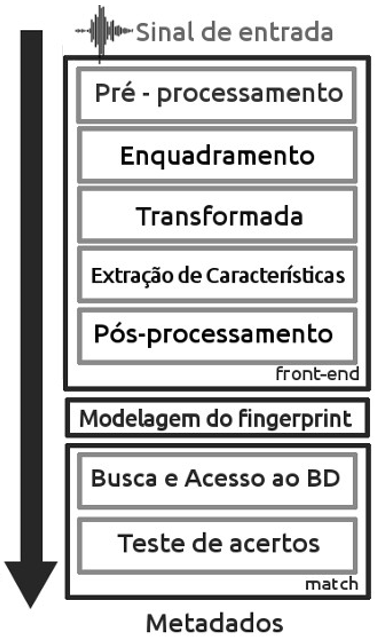
\includegraphics[scale=0.50]{figs/arquitetura.png}
\label{f.diagrama}
\legend{\small Fonte: Elaborada pelo autor.}
\end{figure}

\subsection{Pré-processamento}
\label{ss.preprocessamento}

Para que o processamento e que a extração de características tome o menor tempo computacional possível, o sinal passará por um filtro que removerá dados que não interessam à extração de características, segundo \citeauthoronline{canoetal05} (\citeyear{canoetal05}, tradução nossa): convertendo para o formato de 16 bits PCM\footnote{Pulse-code modulation: método usado para representação digital de sinais analógicos.}, agrupando através da média os canais esquerdo e direito em uma taxa de amostragem variando de 5 a 44,1 kHz.

\subsection{Enquadramento}
\label{ss.enquadramento}

O enquadramento adapta a amostragem para o que será utilizado. \citeauthoronline{canoetal05} (\citeyear{canoetal05}) definem o enquadramento dizendo que:

\begin{quotation}
``Um pressuposto fundamental na medição das características é que o sinal pode ser considerado como estacionário em um intervalo de alguns milissegundos. Portanto, o sinal é dividido em quadros de dimensão comparável à velocidade de variação dos eventos acústicos subjacentes. O número de quadros computados por segundo é chamado de taxa de quadros. Uma função de janela é aplicada a cada bloco para minimizar as descontinuidades entre o início e o fim. Uma justaposição deve ser aplicada para garantir robustez para o deslocamento (isto é, quando os dados de entrada não forem perfeitamente alinhados). E é necessário equilibrar os valores acima entre a taxa de variação no espectro e complexidade do sistema''
\end{quotation}

\subsection{Transformada}
\label{ss.transformada}

A complexidade do sistema define como será tratado o enquadramento, para que o algoritmo de reconhecimento possa realizar uma melhor classificação dentro das características desejadas.

Os sinais sonoros que observamos são captados em função do tempo, mas ao aplicar transformadas que convertam esses sinais em função da frequência é possível observar particularidades que não podiam ser observadas anteriormente, assim como também é possível fazer um reconhecimento de padrões desses sinais em função da frequência. A transformada de Karhunen-Loève é uma transformada que consegue comprimir de maneira ótima os dados referentes ao sinal  (\citeauthoronline{raok} , \citeyear{raok}), mas depende da função de entrada, tornando o cálculo computacional demasiadamente intensivo. \citeauthoronline{canoetal05} (\citeyear{canoetal05}) também cita a decomposição em valores singulares como uma compressão ótima porém impraticável. Outras transformadas são citadas que podem ser utilizadas para extrair características:

\begin{alineas}

\item Tranformada rápida de Fourier
\item Transformada de Walsh-Hadamard
\item \emph{Modulated Complex Lapped Transform (MCLT)}
\item Transformada Wavelet

\end{alineas}


\subsection{Extração de Características}
\label{ss.extracaocaracteristicas}

Os dados obtidos pela transformada serão novamente transformados de modo que aumente a sua invariânica a distorções do som, como aumento do pitch ou mudança do tempo. Características que fazem parte do objetivo são levadas em conta nessa fase, como frequências relevantes (no caso de extração de voz ou reconhecimento de instrumentos), harmonicidade e ruído (no caso de classificação musical).

\subsection{Pós-processamento}
\label{ss.posprocessamento}

Para complementar os dados absolutos, as variações temporais podem ser adicionadas ao sinal processado, através das derivativas de primeira e segunda ordem.

Os metódos da primeira fase onde o sinal é pré-processado até aqui são agrupados e podem ser classificados como o front-end da obtenção do fingerprint.

\subsection{Modelagem do Fingerprint}
\label{ss.modelagemfingerprint}

A modelagem do fingerprint usualmente recebe uma sequência de vetores de características calculadas quadro a quadro \citeauthoronline{canoetal05} (\citeyear{canoetal05}, tradução nossa). As características que serão usadas para montar o modelo do fingerprint influenciam a forma como o algoritmo irá tratar futuramente a busca dessas características para comparação. Os processos mais simplificados como o de softwares como o \emph{Music-brainz} traduzem as características para um hash de identificação, outros mais complexos armazenam o modelo em um formato de vetor ou matriz bidimensional.

\subsection{Busca e acesso ao BD}
\label{ss.buscabd}

A Busca depende diretamente do modelo definido e do problema a ser resolvido, pois nesse passo é preciso classificar o peso de cada característica extraída e a métrica utilizada para encontrar a distância entre cada fingerprint. O Banco de dados armazena os fingerprints já identificados e pode criar indíces de busca para campos de maior relevância, para diminuir o custo computacional da comparação.

\subsection{Teste de Acertos}
\label{ss.testeacertos}

Para identificação do fingerprint, ele passa por um teste de cálculo da probabilidade de acerto, onde é verificado se pertence ou não ao banco de dados atual, podendo ser classificado como pertencente ou não. Deve-se definir um limite de aceitação para classificar também um dado falso positivo (no caso de um banco de dados muito grande) ou um falso negativo (no caso de dados insuficientes).


\section{Chromaprint}
\label{s.chromaprint}

Segundo \citeauthoronline{chromaprint} (\citeyear{chromaprint}, tradução nossa) a música popular é frequentemente baseada em uma estrutura simples que pode alternar entre versos e um refrão ou acorde repetido. Uma estratégia razoável para selecionar uma representação musical nestes casos mais simples envolve a localização e identificação destas seções que se repetem.

\subsection{PCP - \emph{Pitch Class Profile} }
\label{ss.pcp}

\citeauthoronline{shepard} (\citeyear{shepard}, tradução nossa) diz que uma nota tocada nos remete a várias propriedades de percepção. Uma é o pitch, que é a qualidade do som determinada pela taxa de vibrações que produz; o grau agudo ou grave de um tom. Outra é a similaridade entre os intervalos de pitch, que também são chamadas de  ``cores'' da nota, essa propriedade pode ser classificada como a escala de notas e denominada o \emph{chroma} da nota, ou \emph{pitch class profile}.
\begin{figure}[h]
\caption{\small Illustração da hélice de Shepard sobre percepção do \emph{pitch}. O eixo vertical representa a altura do tom e a dimensão angular representa o \emph{chroma}}
\centering
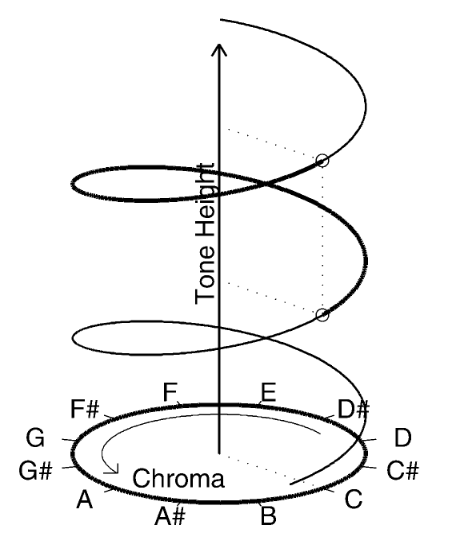
\includegraphics[scale=0.8]{figs/chromaperception.png}
\label{f.chromaperception}
\legend{\small Fonte:  \cite{chromaprint}.}
\end{figure}


\subsection{\emph{Chroma} musical e a música ocidental }
\label{ss.westmusic}

Na teorica musical ocidental o sistema de tons divide cada oitava em doze partes iguais, classificando a frequência de 440Hz como um lá (A), e progredindo a escala logaritmamente a partir dessa frequência até repetir novamente a sensação cromática do lá, alcançada na frequência de 880Hz, esse intervalo entre as duas notas é denominado uma oitava, e dividido em 12 partes iguais, essa divisão é chamada de escala cromática.

\begin{figure}[h]
\caption{\small Representação da escala cromática iniciando em um Dó (C).}
\centering
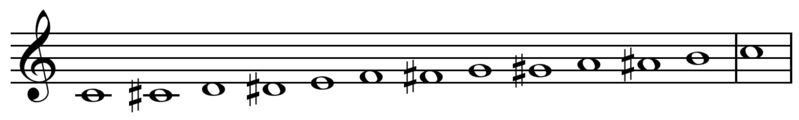
\includegraphics[scale=0.6]{figs/escalacromatica.png}
\label{f.chromaticn}
\legend{\small Fonte:  Elaborada pelo autor.}
\end{figure}

Devido a repetição de frequência e similaridade de notas, podemos representar as notas de uma música em um vetor de 12 posições, um para cada classe de \emph{pitch}. Essa representação nos permite extrair características musicais através de uma DFT\footnote{Discrete Fourier transform - Transformação discreta de Fourier}:

\begin{figure}[h]
\caption{\small Representação colorida de \emph{chroma features}.}
\centering
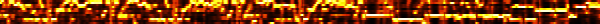
\includegraphics[scale=0.6]{figs/chr.png}
\label{f.chromaticn}
\legend{\small Fonte:  \cite{chromaworks}.}
\end{figure}

\subsection{Comparação de fingerprint por filtro visual.}
\label{ss.visual}

\cite{pasteldeflango} definem um algoritmo de comparação de dois \emph{audio fingerprints} com base em um filtro visual de soma de características. Existem dezesseis tipos de filtros aplicados a uma janela de tamanho de 16x12 pixels, cada filtro é aplicado para capturar diferentes intensidades musicais.

\begin{figure}[h]
\caption{\small Formas de arranjo dos filtros visuais.}
\centering

\includegraphics[scale=1]{figs/filters.png}
\label{f.chromaticn}
\legend{\small Fonte:  \cite{chromaworks}.}
\end{figure}

Segundo \citeauthoronline{chromaworks} (\citeyear{chromaworks}, tradução nossa) para cada filtro é calculada a diferença da soma das áreas brancas com a soma das áreas pretas. Cada filtro tem três coeficientes associados a ele, que guiam como classificar o resultado de 0 a 3. Esse filtros e coeficientes foram selecionados por um algoritmo de aprendizado de máquina, treinado durante o desenvolvimento da biblioteca. 

\begin{figure}[h]
\caption{\small Diferença bit a bit de duas versões da música, uma sem compressão e a outra comprimida em MP3.}
\centering
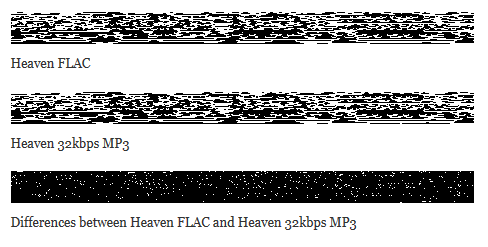
\includegraphics[scale=1]{figs/heavendifferences.png}
\label{f.chromaticn}
\legend{\small Fonte:  \cite{chromaworks}.}
\end{figure}

O resultado dos 16 filtros produzem um inteiro que pode ser codificado em 2 bits, combinando os resultados temos um inteiro de 32 bits, se aplicarmos estes filtros para cada janela dos \emph{chroma features} obtemos um \emph{audio fingerprint} completo.

Com base nesse fingerprint a busca por proximidade em um banco de dados pode ser otimizada para encontrar uma música que esteja mais próxima da música procurada, mesmo que em versões diferentes.

\begin{figure}[h]
\caption{\small Diferença entre as versões originais e instrumentais de duas músicas.}
\centering
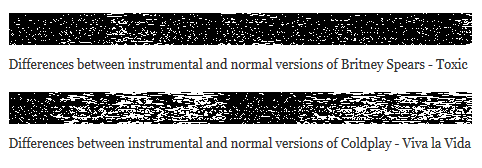
\includegraphics[scale=1]{figs/instrumental.png}
\label{f.chromaticn}
\legend{\small Fonte:  \cite{chromaworks}.}
\end{figure}

\chapter{Metodologia}
\label{c.metodologia}

\section{Métodos e Etapas}
\label{s.metodoseetapas}

Para o desenvolvimento do projeto foi realizado o levantamento bibliográfico de tecnologias existentes e modelos organizacionais referentes à extração de \emph{Audio Fingerprint}, assim como a comparação específica de modelos de ondas sonoras de músicas e melodias.

Com a base teórica definida a etapa seguinte foi aplicar uma estrutura modular que correspondesse ao modelo teórico, para que todas as etapas da extração e reconhecimento do \emph{audio fingerprint} possam ser modificadas sem que alterem o funcionamento geral do processo. Essa estrutura adaptável foi aplicada com base no modelo teórico genérico de reconhecimento de áudio.

A terceira e última etapa foi o desenvolvimento de uma aplicação de reconhecimento específico de músicas, utilizando um cálculo de \emph{audio fingerprint} baseado em representações que levam em conta a repetição de refrões através da análise baseada em altura tonal e \emph{chroma} musical.

\section{Materiais Utilizados}
\label{s.materiaisutilizados}


\subsection{Servidor de desenvolvimento}
\label{s.v8}

Para desenvolvimento do projeto foi utilizada uma máquina externa com 512MB de RAM, Disco SSD com 20GB e Ubuntu 14.04 x64.

\subsection{Github}
\label{s.github}

O Github é ao mesmo tempo um servidor de armazenamento de código e uma rede social onde pode-se submeter modificações, fazer cópias e acompanhar modificações de códigos de outras pessoas. A rede foi essencial para o desenvolvimento deste projeto por armazenar vários sub-módulos e disponibilizar código-fonte para consulta.

\subsection{V8 JavaScript Engine}
\label{s.v8}

V8 é um projeto open-source da Google para interpretação de Javascript, escrito em C++ e utilizado no navegador \emph{Google Chrome}. Ele implementa o ECMAScript e pode ser inserido em aplicações C++ nativas.

\subsection{Node.js}
\label{s.nodejs}

O Node.js é um interpretador \emph{JavaScript} multiplataforma que utiliza o \emph{V8 JavaScript Engine}, foi criado em 2009 por Ryan Dahl e atualmente é utilizado para aplicações variadas. Seu funcionamento \emph{single threaded} simplifica a construção da aplicação, foi escolhido para o desenvolvimento deste projeto por facilitar o desenvolvimento modular e comunicação entre os módulos.

\subsection{npm}
\label{s.npm}

O npm é uma sigla para \emph{node package manager} mas é um gerenciador de pacotes geral que implementa não somente os pacotes de node como também de projetos variados em javascript e outras linguagens. O npm permite a instalação e gerenciamento de pacotes e bibliotecas de maneira facilitada, coordenando as versões utilizadas de acordo com a necessidade do projeto.

\subsection{FFmpeg}
\label{s.ffmpeg}

O FFmpeg é um programa externo multiplataforma utilizado através do node. Ele grava, converte e cria \emph{stream} de vários formatos de áudio e vídeo.

\chapter{Desenvolvimento}
\label{c.desenvolvimento}

\section{Modelo Teórico e estrutura modular}
\label{s.modeloteorico}

Seguindo a abordagem descrita por \citeauthoronline{canoetal05} (\citeyear{canoetal05}) foi desenvolvido um módulo para cada fase dos processos de extração do \emph{audio fingerprint}:

\begin{alineas}

\item Pré-processamento
\item Enquadramento
\item Transformada
\item Extração de características
\item Pós-processamento
\item Modelagem do fingerprint

\end{alineas}

Cada etapa é um módulo independente que passa a informação tratada através de stream de audio ou arquivo para a próxima etapa até a obtenção do \emph{audio fingerprint} final. Uma etapa anterior foi adicionada para extrair o audio de uma fonte web e enviar para o sistema de geração de \emph{audio fingerprint}.


\begin{figure}[h]
\caption{\small Ambiente de desenvolvimento da aplicação do modelo teórico.}
\centering
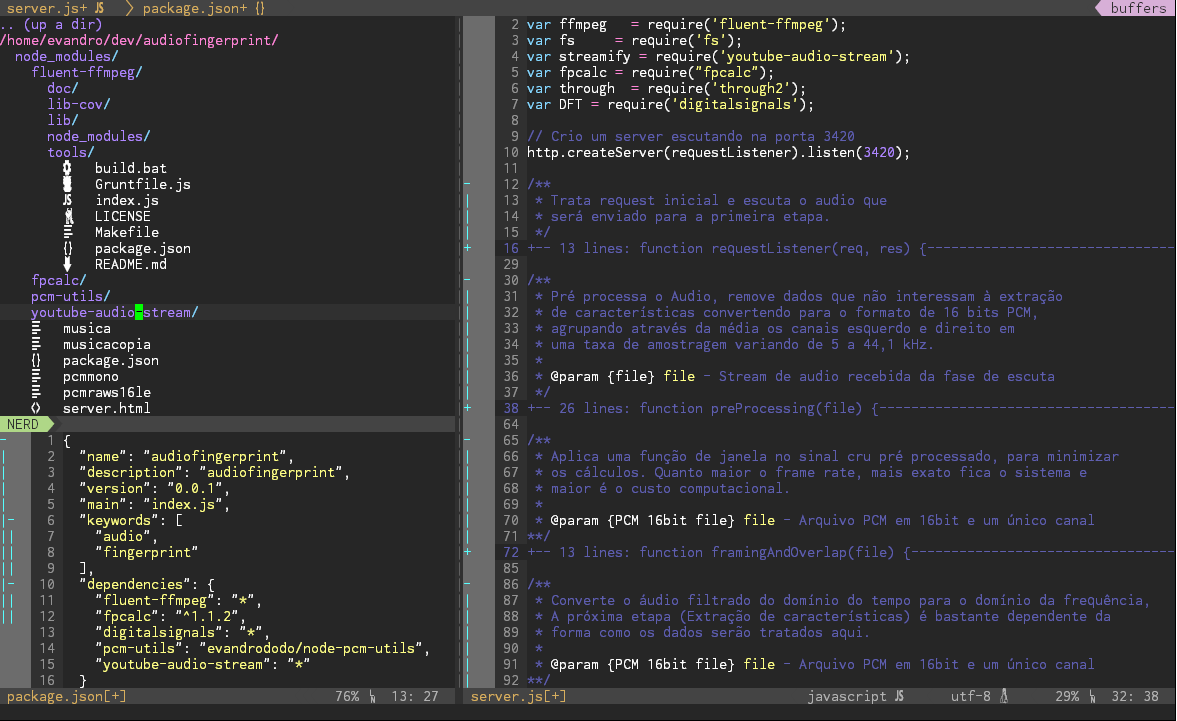
\includegraphics[scale=0.50]{figs/ambientegeral.png}
\label{f.diagrama}
\legend{\small Fonte: Elaborada pelo autor.}
\end{figure}

\subsection{Pré-processamento}
\label{ss.preprocessamento}

Pré processa o Audio, converte para o formato de 16 bits PCM, e agrupa através da média os canais esquerdo e direito em uma taxa de amostragem variando de 5 a 44,1 kHz.
	
\begin{verbatim}
function preProcessing(file) {
    // Cria um stream de leitura com base no arquivo que esá
    //  recebendo a musica em PCM
    var preProcStream = fs.createReadStream(file),
        pcmMono = fs.createWriteStream('pcmmono'),
        musica = '';

    preProcStream.on('data', function(chunk) {
        console.log(chunk.length);
        musica += chunk;
    });

    preProcStream.on('end', function(chunk) {
        console.log('Iniciando conversão para PCM...');
        ffmpeg(__dirname + '/musicacopia')
        .format('pulse')
        .audioChannels(1)
        .output(__dirname + '/pcmmono')
        .on('end', function() {
            console.log('Música convertida para PCM 16bits Mono');
            framingAndOverlap(__dirname + '/pcmmono');
        })
        .run();
    });
} 
\end{verbatim}	

\subsection{Enquadramento}
\label{ss.enquadramento}

Aplica uma função de janela no sinal cru pré processado, para minimizar os cálculos. Quanto maior o frame rate, mais exato fica o sistema e maior é o custo computacional.

\begin{verbatim}
function framingAndOverlap(file) {
  var preProcStream = fs.createReadStream(file),
      frameSize = 4096, 
      overlap = 75, //porcentagem
      fao = new framingAndOverlap();
      
      fao.size(frameSize).overlap(overlap).run(preProcStream);
      transformada(file);
}
\end{verbatim}


\subsection{Transformada}
\label{ss.transformada}

Converte o Audio filtrado do domí­nio do tempo para o domí­nio da frequência,  a próxima etapa (Extração de caracterí­sticas) é bastante dependente da forma como os dados serão tratados aqui.
	
\begin{verbatim}
function transformada(file) {
  var procSinal = fs.createReadStream(file),
      dftStream = fs.createWriteStream(__dirname + '/dft'),
      dft = new DFT(1024, 44100);
  dft.forward(procSinal);
  var spectrum = dft.spectrum;
  spectrum.pipe(dftStream);
  extracao(dtStream);
}
\end{verbatim}


\subsection{Extração de Características}
\label{ss.extracaocaracteristicas}

A extração de características deve ser ajustada para a finalidade desejada do \emph{audio fingerprint}. No caso de reconhecimento de voz ou instrumentos, os dados mais relevantes são os referentes às frequências com maior indíce de repetição (harmônicas presentes). No caso de reconhecimento de músicas os dados relevantes são a repetições de refrões, melodia e \emph{chroma} musical.

\begin{verbatim}
function extracao(stream) {
  var sinalfreq = fs.createReadStream(stream);

    // Análise simplificada do sinal sonoro: contando as frequencias
    // que mais se repetem (harmonicas de instrumento)
    sinalfreq.on('end', function(chunk) {
        console.log('Contando frequências do sinal e agrupando');
        var coordFN = sinalfreq;
        // Envia a contagem para o pós processamento como um vetor
        // de distância em N dimensões, sendo N o número de 
        // frequências disponíveis
        posprocess(coordFN);
    });
}
\end{verbatim}


\subsection{Pós-processamento}
\label{ss.posprocessamento}

Para gerar um fingerprint o dado com as características relevantes deve ser normalizado e pode ser simplificado atraves de derivadas de primeira e segunda ordem.

\begin{verbatim}
function posprocess(coords) {
  var maxFreq = -11000,
      minFreq = 11000;
   for(int i=0;i<coords.length;i++) {
       if(coords[i]<minFreq) {
           minFreq = coords[i];
       }
       if(coords[i]>maxFreq) {
           maxFreq = coords[i];
       }
    }
    var amplitude = maxFreq - minFreq,
       intervalo = amplitude/36; //26 letras e 10 numeros
    // Normalizando o sinal para 36 representações
   for(int i=0;i<coords.length;i++) {
       coords[i] = Math.round(coords[i]/intervalo);
    }
    modeling(coords);
}
\end{verbatim}

\subsection{Modelagem do Fingerprint}
\label{ss.modelagemfingerprint}

A modelagem do fingerprint usualmente recebe uma sequência de vetores de características. Através desse vetor é gerado um hash de identificação.

\begin{verbatim}
function modeling(coords) {
    var simbolos = ["a", "b", "c", "d", "e", "f", "g", "h", "i", "j", "k", "l",
     "m", "n", "o",     "p", "q", "r", "s", "t", "u", "v", "w", "x", "y", "z",
      "0", "1", "2", "3", "4", "5", "6", "7", "8", "9"];
        hash = ""';
   for(int i=0;i<coords.length;i++) {
     hash = hash + simbolos[coords[i]];
    }
    console.log('Hash de identificação:');
    console.log(hash);
}
\end{verbatim}

\section{Geração de hash com modelo de contagem de frequências}
\label{s.teste}

Com base no algoritmo modular desenvolvido foi gerado um hash para teste de eficiência de processamento, esses módulos podem ser modificados para atender vários modelos de \emph{audio fingerprint}. Como exemplo as transformadas DFT podem ser substítuidas por transformadas Wavelet e o vetor pode ser resumido à derivativa de primeira ordem, dependendo da finalidade da aplicação.

\begin{figure}[h]
\caption{\small Teste de geração de hash simples.}
\centering
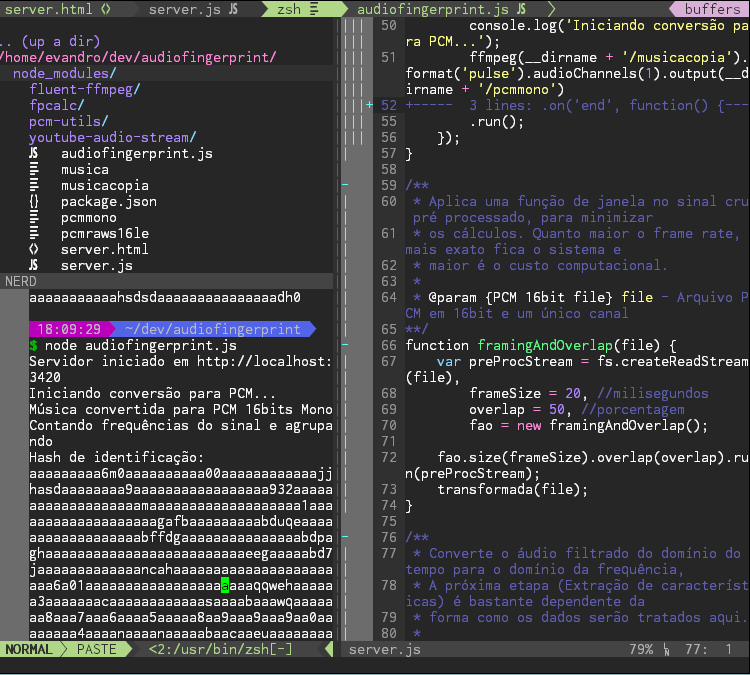
\includegraphics[scale=0.75]{figs/execucao.png}
\label{f.execucao}
\legend{\small Fonte: Elaborada pelo autor.}
\end{figure}

\section{Base de dados e reconhecimento de músicas}
\label{s.basedados}

Para catálogo de músicas e artistas existentes foi utilizado o banco de dados da MusicBrainz, que disponibiliza um script de backup e criação de um banco \emph{PostgreSQL}. Os dados deste banco estão em domínio público e a MusicBrainz disponibiliza também um servidor que sincroniza os dados à cada uma hora.

\begin{figure}[h]
\caption{\small Organização do banco de dados do MusicBrainz.}
\centering
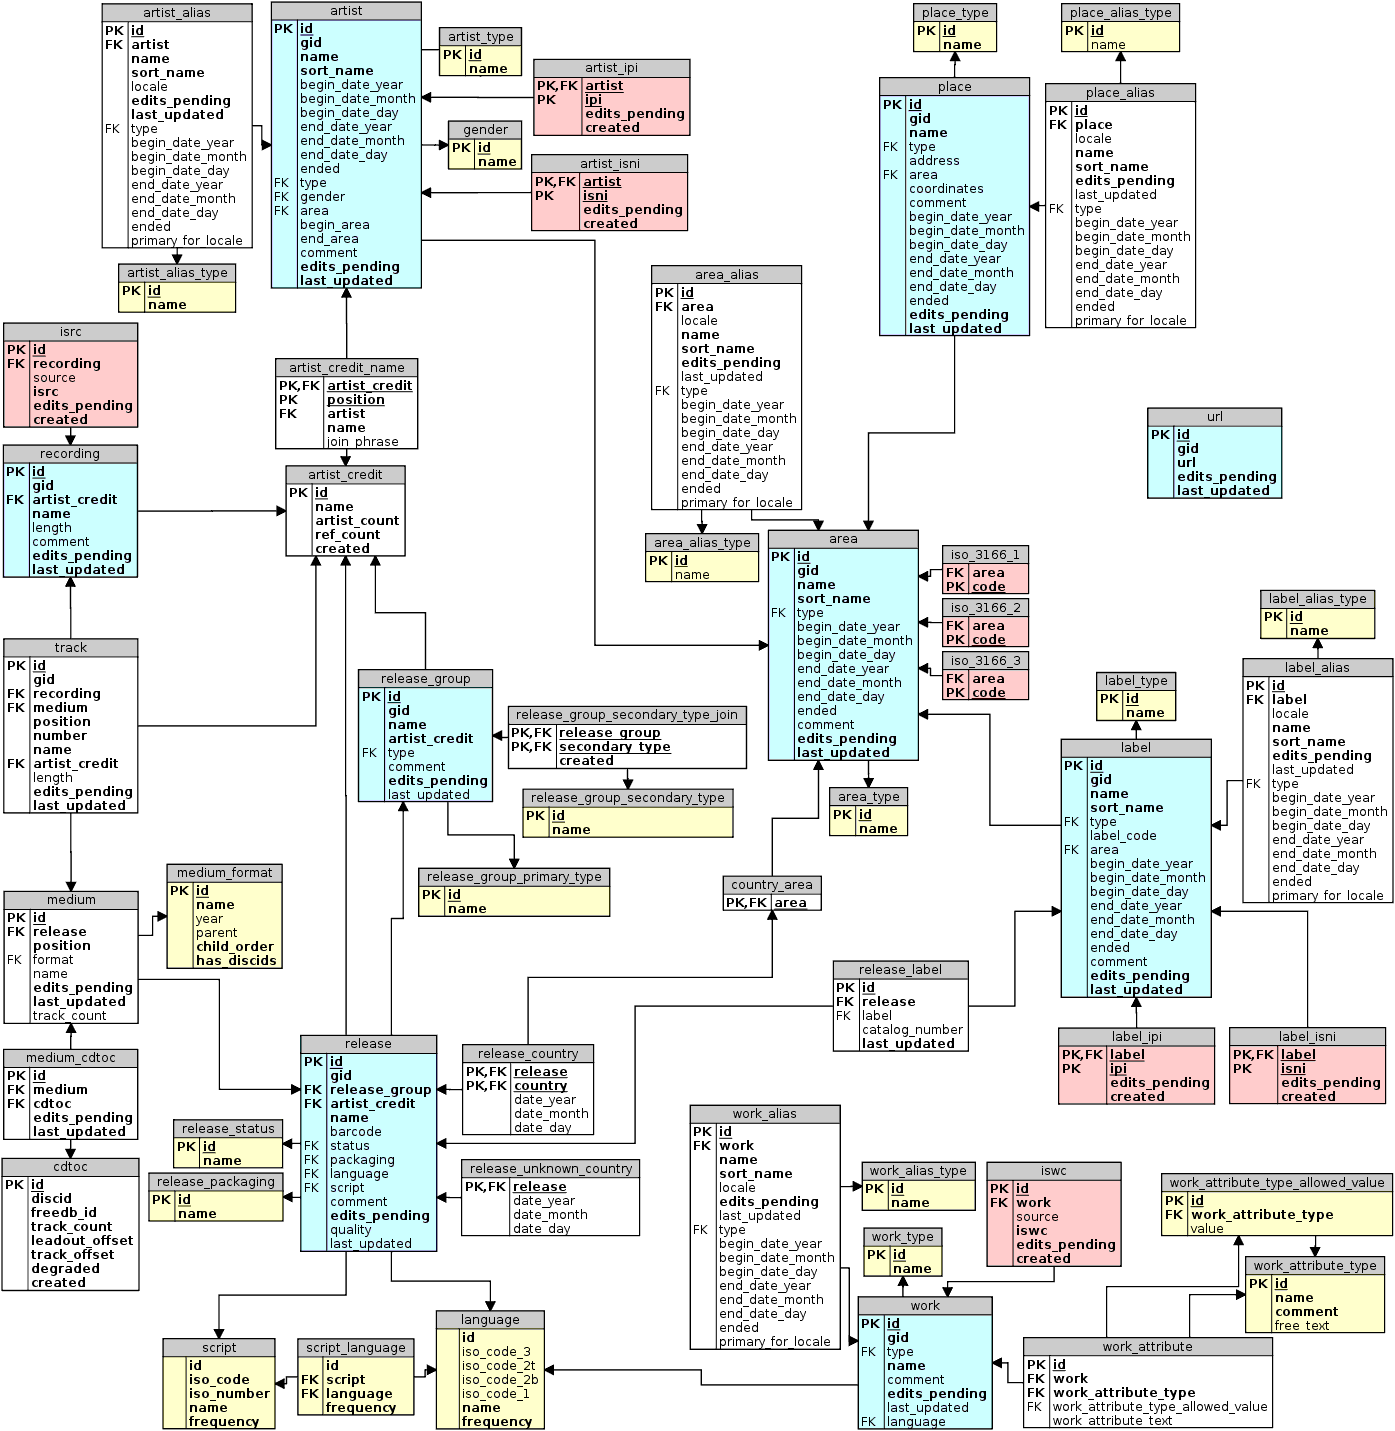
\includegraphics[scale=0.40]{figs/musicbrainzschema.png}
\label{f.musicbrainz}
\legend{\small Fonte: \cite{musicbrainzcite}.}
\end{figure}
 
 Inicialmente foi utilizado um banco de dados local para consulta e treinamento do algoritmo de hash, na fase final de reconhecimento de música a consulta remota em outra máquina se mostrou mais eficiente.
 
\section{Geração de hash \emph{Chroma-based}}
\label{s.hashchroma}

Para a geração de hash para consulta de músicas foi utilizado o algoritmo de \emph{Chromaprint}, descrito na seção \ref{s.chromaprint}. O algoritmo gera um hash representado em caracteres alfanuméricos que pode ser utilizado para consulta nos bancos de dados disponíveis. 

\begin{figure}[h]
\caption{\small Geração de hash com algoritmo de \emph{Chromaprint}.}
\centering
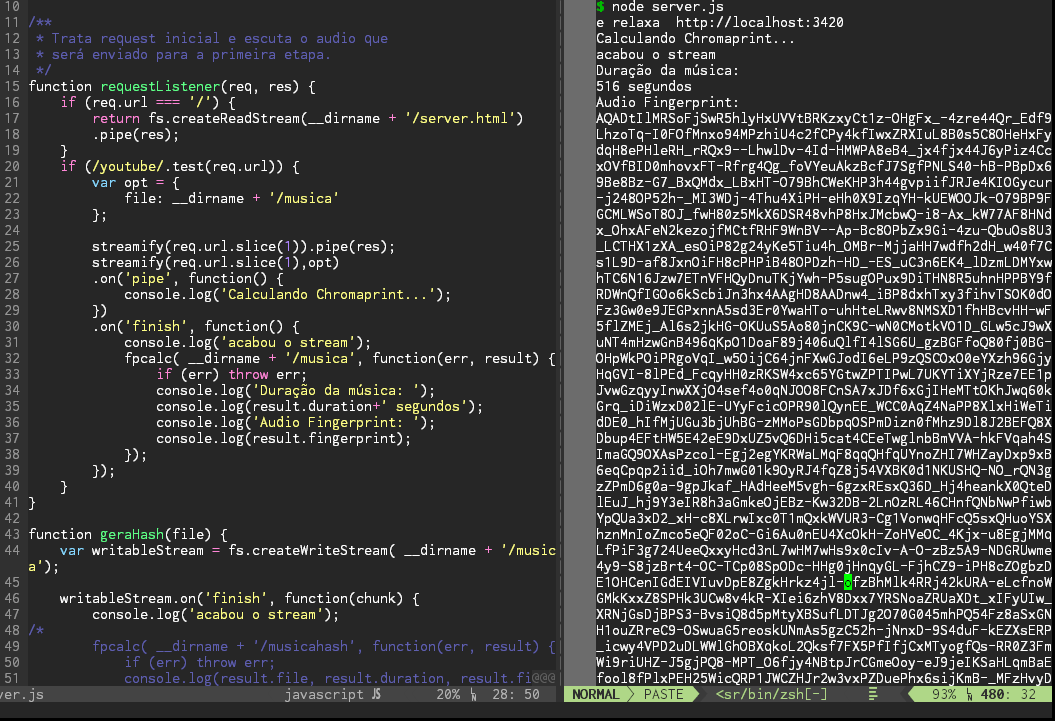
\includegraphics[scale=0.60]{figs/hashchromaprint.png}
\label{f.musicbrainz}
\legend{\small Fonte: Elaborada pelo autor.}
\end{figure}
 

\section{Busca, acesso e teste de acertos}
\label{s.buscanobd}

Com o hash representando o \emph{audio fingerprint} o último passo necessário para o reconhecimento é a consulta no banco de dados. Para a busca, acesso e teste de acertos foi utilizada a base disponibilizada \cite{musicbrainzcite} e o  \emph{web service} da AcoustID, com acesso e comparação através do hash enviado:

\begin{figure}[h]
\caption{\small Busca no banco de dados.}
\centering
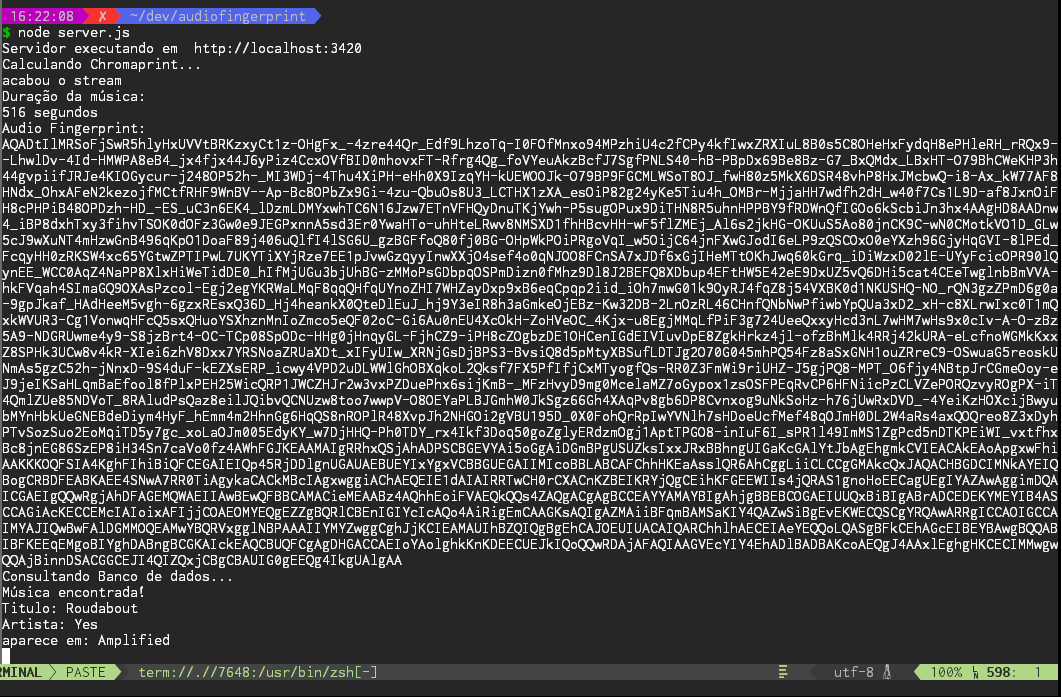
\includegraphics[scale=0.60]{figs/yes.png}
\label{f.musicbrainz}
\legend{\small Fonte: Elaborada pelo autor.}
\end{figure}
 
\chapter{Conclusão}
\label{c.conclusao}

O objetivo deste projeto foi desenvolver um aplicativo modular que possa ser usado como ferramenta para o desenvolvimento de tecnologias web disponíveis atualmente, assim como o de propagar o conhecimento e facilitar a compreensão do assunto que envolve o tema de reconhecimento de sons. 

O código de todo o projeto desenvolvido foi disponibilizado no \emph{Github}, sob licença MIT, que garante permissão de cópia, reprodução, distribuição, publicação e venda para qualquer pessoa, reforçando o caráter público e comunitário. Para acesso ao código fonte do projeto e documentos utilizados durante o desenvolvimento acesse \url{https://github.com/evandrododo/piratify}.

Todas as etapas foram essenciais para a aplicação, e por se tratar de uma tecnologia em constante desenvolvimento a comunidade de programadores envolvidos contribuiu com as bibliotecas utilizadas tanto antes do início do projeto como durante, aplicando correções necessárias e modificações para melhoria de desempenho. O Resultado final foi uma aplicação de um modelo teórico simplificado e um protótipo funcional de reconhecimento de audio.


% ----------------------------------------------------------
% ELEMENTOS PÓS-TEXTUAIS
% ----------------------------------------------------------
\postextual
% ----------------------------------------------------------
	
% ----------------------------------------------------------
% Referências bibliográficas
% ----------------------------------------------------------
\pagestyle{empty}
\bibliography{references} % o arquivo de bibliografia deve ser importando nessa linha sem o .bib

% ----------------------------------------------------------
% Glossário
% ----------------------------------------------------------
%
% Consulte o manual da classe abntex2 para orientações sobre o glossário.
%
%\glossary

%---------------------------------------------------------------------
% INDICE REMISSIVO
%---------------------------------------------------------------------
\phantompart
\printindex
%---------------------------------------------------------------------

\end{document}
